\documentclass[12pt]{article}
\usepackage{amsmath}
\usepackage{amssymb}
\usepackage{graphicx}
\usepackage{hyperref}


\title{Reproduction Report on VMAS: A Vectorized Multi-Agent Simulator for Collective Robot Learning}
\author{}
\date{}

\begin{document}

\maketitle

\section{Introduction}
This report details the reproduction process of the paper "VMAS: A Vectorized Multi-Agent Simulator for Collective Robot Learning". It includes explanations on key components, algorithms, and code comments based on the original source code.

\section{Reading Paper \& Key Steps Code Comments}

\subsection{Core Architecture Design}

\subsubsection{World Class}
\begin{verbatim}
class World:  # vmas/simulator/core.py
    """
    World Class - Core of the entire simulator
    Functions:
    1. Manages all entities (agents and landmarks)
    2. Handles physics engine updates
    3. Handles collision detection
    4. Supports vectorized parallel environments
    5. Customizable gravity, friction, and other physical parameters
    """
\end{verbatim}

\subsubsection{Environment Class}
\begin{verbatim}
class Environment:  # vmas/simulator/environment/environment.py
    """
    Environment Class - Manages multi-agent environments
    Functions:
    1. Scene management and reset
    2. Action and observation space definitions
    3. Reward calculation
    4. State updates
    5. Rendering and visualization
    """
\end{verbatim}

\subsubsection{Agent Class}
\begin{verbatim}
class Agent:  # vmas/simulator/core.py
    """
    Agent Class
    Functions:
    1. State management (position, velocity, acceleration)
    2. Action execution
    3. Collision handling
    4. Sensor integration
    """
\end{verbatim}

\subsection{Physics Engine Implementation}

\subsubsection{Shape Class}
\begin{verbatim}
class Shape:  # vmas/simulator/core.py
    """
    Shape Base Class
    Supports:
    1. Sphere
    2. Box
    3. Line
    """
\end{verbatim}

\subsubsection{Dynamics Class}
\begin{verbatim}
class Dynamics:  # vmas/simulator/dynamics/common.py
    """
    Dynamics Model
    Implements:
    1. Omnidirectional movement
    2. Differential drive
    3. Bicycle model
    4. Drone model
    """
\end{verbatim}

\subsubsection{Collision Detection}
\begin{verbatim}
def _get_closest_points():  # vmas/simulator/physics.py
    """
    Collision Detection Algorithm
    Supports:
    1. Sphere-sphere collision
    2. Sphere-box collision
    3. Sphere-line segment collision
    4. Line segment-line segment collision
    """
\end{verbatim}

\subsection{Scene System}

\subsubsection{Base Scenario Class}
\begin{verbatim}
class BaseScenario:  # vmas/simulator/scenario.py
    """
    Base Scenario Class
    Key Methods:
    1. make_world() - Create and initialize the world
    2. reset_world_at() - Reset specific environment states
    3. observation() - Define the observation space
    4. reward() - Define the reward function
    5. done() - Define termination conditions
    """
\end{verbatim}

\subsubsection{Football Scenario}
\begin{verbatim}
class Football(BaseScenario):  # vmas/scenarios/football.py
    """
    Football Scenario
    Features:
    1. Multi-agent cooperation
    2. Ball physics simulation
    3. Match rules implementation
    """
\end{verbatim}

\subsubsection{Navigation Scenario}
\begin{verbatim}
class Navigation(BaseScenario):  # vmas/scenarios/navigation.py  
    """
    Navigation Scenario
    Features:
    1. Path planning
    2. Obstacle avoidance
    3. Goal tracking
    """
\end{verbatim}

\subsection{Sensor System}

\subsubsection{Sensor Class}
\begin{verbatim}
class Sensor:  # vmas/simulator/sensors.py
    """
    Sensor Base Class
    Supports:
    1. LIDAR (Laser Radar)
    2. Communication Channel
    3. Camera
    4. GPS
    """
\end{verbatim}

\subsubsection{Controller Class}
\begin{verbatim}
class Controller:  # vmas/simulator/controllers/
    """
    Controller
    Implements:
    1. PID control
    2. Velocity control
    3. Position control
    """
\end{verbatim}

\subsection{Vectorization Implementation}

\subsubsection{TorchVectorizedObject Class}
\begin{verbatim}
class TorchVectorizedObject:  # vmas/simulator/core.py
    """
    Vectorized Base Class
    Functions:
    1. Batch parallel environments
    2. GPU acceleration support
    3. Automatic differentiation
    4. Tensor operations
    """
\end{verbatim}

\subsubsection{Vectorized Physics Function}
\begin{verbatim}
def vectorized_physics():  # vmas/simulator/physics.py
    """
    Vectorized Physics Computation
    Implements:
    1. Batch collision detection
    2. Parallel state updates
    3. GPU acceleration
    """
\end{verbatim}

\subsection{Rendering System}

\subsubsection{Viewer Class}
\begin{verbatim}
class Viewer:  # vmas/simulator/rendering.py
    """
    Renderer
    Functions:
    1. 2D scene drawing
    2. Agent visualization
    3. Debug information display
    4. Interactive controls
    """
\end{verbatim}

\subsubsection{Render Function}
\begin{verbatim}
def render():  # vmas/simulator/environment/environment.py
    """
    Rendering Process
    1. Scene drawing
    2. Agent state updates
    3. Collision display
    4. UI elements
    """
\end{verbatim}

\subsection{Training Interface}
\begin{verbatim}
# Standard Reinforcement Learning Interface
"""
Compatible with:
1. OpenAI Gym
2. Gymnasium
3. RLlib
4. TorchRL

Standardized:
1. Action space
2. Observation space
3. Reward function
4. Reset function
"""
\end{verbatim}

\section{Task Reproduction: Balance Scenario}

\subsection{CPPO (Centralized-Planning PPO) - \texttt{train\_balance\_cppo.py}}

\subsubsection{Centralized Actor Network Definition}
\begin{verbatim}
class CentralizedActor(nn.Module):
    def __init__(self, obs_dim, action_dim, n_agents, hidden_dim=512):
        super(CentralizedActor, self).__init__()
        self.n_agents = n_agents
        # Calculate the total observation and action dimensions
        total_obs_dim = obs_dim * n_agents  
        # Total dimension of all agents' observations
        total_action_dim = action_dim * n_agents  
        # Total dimension of all agents' actions
        
        # Construct feature extraction network
        self.net = nn.Sequential(
            nn.Linear(total_obs_dim, hidden_dim),
            nn.LayerNorm(hidden_dim),
            nn.Tanh(),
            nn.Linear(hidden_dim, hidden_dim),
            nn.LayerNorm(hidden_dim),
            nn.Tanh(),
            nn.Linear(hidden_dim, hidden_dim // 2),
            nn.LayerNorm(hidden_dim // 2),
            nn.Tanh(),
        )
        
        # Action distribution parameter layers
        self.mean_layer = nn.Linear(hidden_dim // 2, total_action_dim)  
        # Output action mean
        self.log_std = nn.Parameter(torch.zeros(1, total_action_dim) - 0.5)  
        # Learnable standard deviation
        
        # Apply orthogonal initialization
        for layer in self.net:
            if isinstance(layer, nn.Linear):
                nn.init.orthogonal_(layer.weight, gain=np.sqrt(2))
                nn.init.constant_(layer.bias, 0)
        nn.init.orthogonal_(self.mean_layer.weight, gain=0.01)
        nn.init.constant_(self.mean_layer.bias, 0)
\end{verbatim}

\subsubsection{Centralized Critic Network Definition}

\begin{verbatim}
class CentralizedCritic(nn.Module):
    def __init__(self, obs_dim, n_agents, hidden_dim=512):
        super(CentralizedCritic, self).__init__()
        total_obs_dim = obs_dim * n_agents  
        # Total dimension of all agents' observations
        
        # Construct value estimation network
        self.net = nn.Sequential(
            nn.Linear(total_obs_dim, hidden_dim),
            nn.LayerNorm(hidden_dim),
            nn.Tanh(),
            nn.Linear(hidden_dim, hidden_dim),
            nn.LayerNorm(hidden_dim),
            nn.Tanh(),
            nn.Linear(hidden_dim, hidden_dim // 2),
            nn.LayerNorm(hidden_dim // 2),
            nn.Tanh(),
            nn.Linear(hidden_dim // 2, 1)  # Output state value
        )
        
        # Use orthogonal initialization
        for layer in self.net:
            if isinstance(layer, nn.Linear):
                nn.init.orthogonal_(layer.weight, gain=np.sqrt(2))
                nn.init.constant_(layer.bias, 0)
\end{verbatim}

\subsubsection{CPPO Trainer Implementation}

\begin{verbatim}
class CPPOTrainer:
    def __init__(self, env, device="cpu"):
        self.env = env
        self.device = device
        self.n_agents = len(env.agents)
        
        # Get environment information
        obs = env.reset()
        self.obs_dim = obs[0].shape[1]  
        # Observation dimension of a single agent
        self.action_dim = env.agents[0].action_size  
        # Action dimension of a single agent
        
        # Create Actor and Critic networks
        self.actor = CentralizedActor(self.obs_dim, self.action_dim, \\
        self.n_agents).to(device)
        self.critic = CentralizedCritic(self.obs_dim, self.n_agents).to(device)
        
        # Create optimizers
        self.actor_optimizer = optim.Adam(self.actor.parameters(), lr=3e-4)
        self.critic_optimizer = optim.Adam(self.critic.parameters(), lr=1e-3)
        
        # PPO hyperparameters
        self.clip_param = 0.2  # PPO clipping parameter
        self.ppo_epochs = 15  # Training epochs per batch
        self.num_mini_batches = 4  # Number of mini-batches
        self.value_loss_coef = 0.5  # Value loss coefficient
        self.entropy_coef = 0.05  # Entropy regularization coefficient
        self.max_grad_norm = 0.5  # Gradient clipping threshold
        self.gamma = 0.99  # Discount factor
        self.gae_lambda = 0.95  # GAE parameter
        
        # Experience buffers
        self.observations = []  # Store observations
        self.actions = []  # Store actions
        self.rewards = []  # Store rewards
        self.values = []  # Store value estimates
        self.log_probs = []  # Store log-probabilities of actions
        self.dones = []  # Store termination flags
\end{verbatim}

\subsubsection{Action Selection and Sampling}

\begin{verbatim}
def select_actions(self, obs_list):
    with torch.no_grad():
        # Get action distribution parameters
        mean, std = self.actor(obs_list)
        # Sample actions
        dist = Normal(mean, std)
        actions = dist.sample()
        actions = torch.clamp(actions, -1.0, 1.0)  # Restrict action range
        log_probs = dist.log_prob(actions)
        entropy = dist.entropy().mean()
        
        # Split actions for individual agents
        action_dim = mean.shape[1] // self.n_agents
        actions_list = torch.split(actions, action_dim, dim=1)
        log_probs_list = torch.split(log_probs, action_dim, dim=1)
        
        # Get state value estimates
        value = self.critic(obs_list)
        
        return actions_list, log_probs_list, value, entropy
\end{verbatim}

\subsubsection{GAE Calculation Implementation}

\begin{verbatim}
def compute_gae(self):
    T = len(self.rewards)
    num_envs = self.rewards[0].shape[0]
    advantages = torch.zeros(T, num_envs, 1, device=self.device)
    returns = torch.zeros(T, num_envs, 1, device=self.device)
    last_gae_lam = torch.zeros(num_envs, 1, device=self.device)
    
    # Backward GAE calculation
    for t in reversed(range(T)):
        if t == T - 1:
            next_value = torch.zeros_like(self.values[0])
        else:
            next_value = self.values[t + 1]
        
        # Calculate TD-error
        delta = self.rewards[t] + self.gamma * next_value * \\
        (1 - self.dones[t]) - self.values[t]
        # Calculate GAE
        advantages[t] = last_gae_lam = delta + self.gamma * self.gae_lambda \\
        * (1 - self.dones[t]) * last_gae_lam
        # Calculate returns
        returns[t] = advantages[t] + self.values[t]
    
    # Standardize advantages
    advantages = (advantages - advantages.mean()) / (advantages.std() + 1e-8)
    
    return advantages, returns
\end{verbatim}

\subsubsection{Implementing Policy Update}

\begin{verbatim}
def update(self):
    # Compute GAE and returns
    advantages, returns = self.compute_gae()
    
    # Prepare training data
    obs_batch = [torch.cat([obs[i] for obs in self.observations]) for \\
    i in range(self.n_agents)]
    actions_batch = [torch.cat([actions[i] for actions in self.actions]) for \\
    i in range(self.n_agents)]
    old_log_probs_batch = [torch.cat([log_probs[i] for log_probs \\
    in self.log_probs]) for i in range(self.n_agents)]
    
    batch_size = len(self.observations) * self.rewards[0].shape[0]
    mini_batch_size = batch_size // self.num_mini_batches
    
    # Multiple rounds of policy iteration
    for i in range(self.ppo_epochs):
        # Generate random indices
        indices = torch.randperm(batch_size)
        
        for start in range(0, batch_size, mini_batch_size):
            end = start + mini_batch_size
            mb_indices = indices[start:end]
            
            # Get mini-batch data
            mb_obs = [obs[mb_indices] for obs in obs_batch]
            mb_actions = [actions[mb_indices] for actions in actions_batch]
            mb_old_log_probs = [old_log_probs[mb_indices] for old_log_probs \\
            in old_log_probs_batch]
            mb_advantages = advantages[mb_indices]
            mb_returns = returns[mb_indices]
            
            # Compute new action distributions
            mean, std = self.actor(mb_obs)
            dist = Normal(mean, std)
            new_log_probs = dist.log_prob(torch.cat(mb_actions, dim=1))
            entropy = dist.entropy().mean()
            
            # Compute the policy ratio and loss
            new_log_probs_list = torch.split(new_log_probs, self.action_dim, \\
            dim=1)
            ratios = [(torch.exp(new_log_probs - old_log_probs)) for \\
            new_log_probs, old_log_probs in zip(new_log_probs_list, \\
            mb_old_log_probs)]
            surr1 = [ratio * mb_advantages for ratio in ratios]
            surr2 = [torch.clamp(ratio, 1.0 - self.clip_param, 1.0 + \\
            self.clip_param) * mb_advantages for ratio in ratios]
            actor_loss = -torch.mean(torch.stack([torch.min(s1, s2).mean() \\
            for s1, s2 in zip(surr1, surr2)]))
            
            # Compute value loss
            value_pred = self.critic(mb_obs)
            value_loss = 0.5 * ((mb_returns - value_pred) ** 2).mean()
            
            # Compute total loss
            loss = actor_loss + self.value_loss_coef * value_loss - \\
            self.entropy_coef * entropy
            
            # Update networks
            self.actor_optimizer.zero_grad()
            actor_loss.backward()
            torch.nn.utils.clip_grad_norm_(self.actor.parameters(), \\
            self.max_grad_norm)
            self.actor_optimizer.step()
            
            self.critic_optimizer.zero_grad()
            value_loss.backward()
            torch.nn.utils.clip_grad_norm_(self.critic.parameters(), \\
            self.max_grad_norm)
            self.critic_optimizer.step()
\end{verbatim}

\subsubsection{Implementing the Training Loop}

\begin{verbatim}
def train_episode(self):
    obs = self.env.reset()
    episode_reward = 0
    done = False
    
    while not done:
        # Select actions
        actions_list, log_probs_list, value, _ = self.select_actions(obs)
        
        # Store transition data
        self.store_transition(
            obs,
            actions_list,
            torch.zeros(self.env.num_envs, 1, device=self.device),
            value,
            log_probs_list,
            torch.zeros(self.env.num_envs, 1, device=self.device)
        )
        
        # Take action
        next_obs, rewards, dones, _ = self.env.step(actions_list)
        done = any(d.any() for d in dones)
        
        # Update rewards and states
        mean_reward = torch.stack([r.mean(dim=0) for r in rewards]).mean() * 100
        self.rewards[-1] = mean_reward.expand(self.env.num_envs, 1)
        self.dones[-1] = torch.full((self.env.num_envs, 1), \\
        float(done), device=self.device)
        episode_reward += mean_reward.item()
        
        obs = next_obs
    
    # Update policy
    actor_loss, value_loss, entropy = self.update()
    
    return actor_loss, value_loss, entropy, episode_reward
\end{verbatim}

This is the implementation process of the CPPO algorithm. The main features are as follows:

1. Centralized Training: Both the Actor and Critic networks receive the joint observations of all agents.A single network processes the information from all agents.

2. Independent Execution: Actions are split and distributed to individual agents.Each agent independently executes its action.

3. PPO Characteristics: Policy updates are constrained using a clipping mechanism to limit step size.The Generalized Advantage Estimation (GAE) is used to compute the advantage function.Multiple rounds of policy iteration are applied.Entropy regularization is applied to promote exploration.

4. Other Features: LayerNorm is used to improve training stability.Orthogonal initialization is applied to avoid gradient issues.Gradient clipping is used to prevent large updates.The advantage function is normalized.

The reward curve is shown below:

\begin{figure}[h]
    \centering
    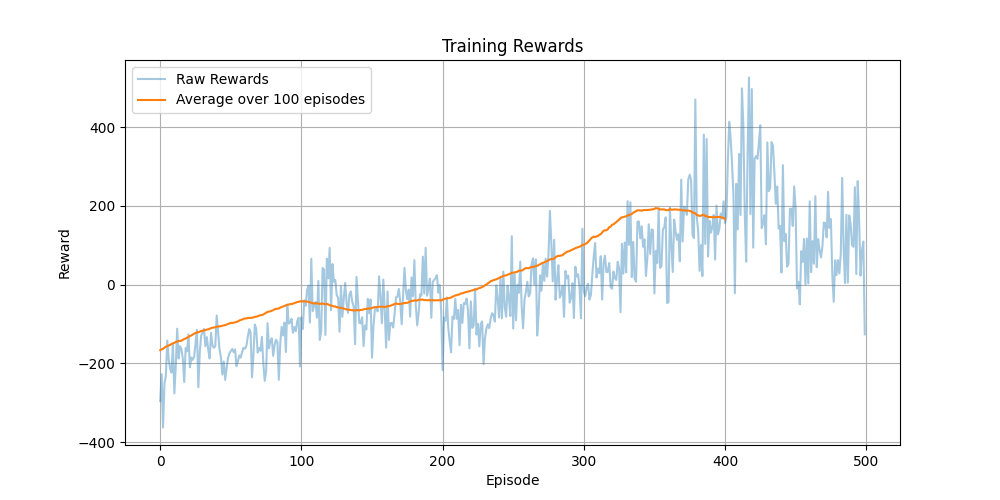
\includegraphics[width=0.7\textwidth]{cppo_training_rewards.png}
    \caption{CPPO Training Rewards}
    \label{fig:cppo_rewards}
\end{figure}

The following are the results from the paper:

\begin{figure}[h]
    \centering
    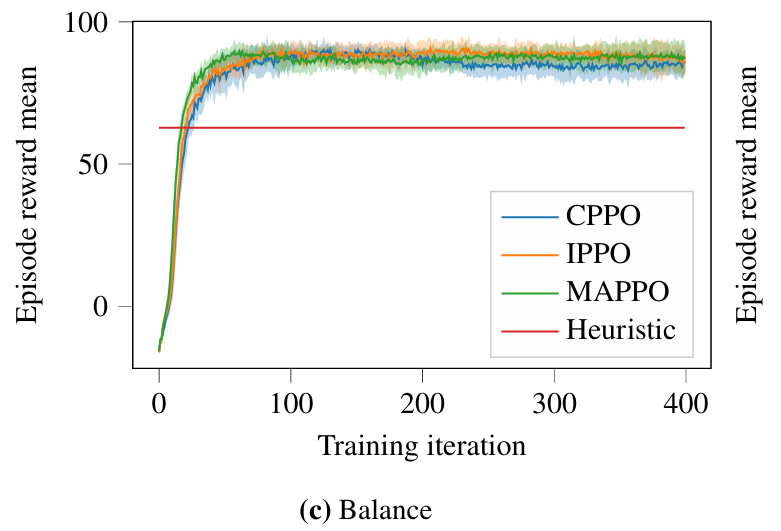
\includegraphics[width=0.7\textwidth]{training_rewards.png}
    \caption{Training Rewards from the Paper}
    \label{fig:paper_rewards}
\end{figure}

The specific training log can be found in the root directory file \texttt{cppo\_training\_log.txt}. The trained models are also saved as \texttt{cppo\_best\_model.pth} and \texttt{cppo\_final\_model.pth}, which are located in the project root directory.

Comparison and Analysis of the Two Reward Curves:

The results from the paper (\ref{fig:paper_rewards}) show faster convergence, stabilizing after approximately 50 iterations. After convergence, there are minimal fluctuations, maintaining a stable level around 90. In contrast, the reproduction results (\ref{fig:cppo_rewards}) show slower convergence, requiring around 300 episodes to stabilize. After convergence, there are greater fluctuations, and the average reward (orange line) eventually stabilizes around 200.

\subsection{MAPPO (Multi-Agent PPO) - \texttt{train\_balance\_mappo.py}}

\subsubsection{Actor Network Implementation}

\begin{verbatim}
class Actor(nn.Module):
    def __init__(self, obs_dim, action_dim, hidden_dim=256):
        super(Actor, self).__init__()
        # Feature extraction network
        self.net = nn.Sequential(
            nn.Linear(obs_dim, hidden_dim),
            nn.LayerNorm(hidden_dim),
            nn.Tanh(),
            nn.Linear(hidden_dim, hidden_dim),
            nn.LayerNorm(hidden_dim),
            nn.Tanh(),
            nn.Linear(hidden_dim, hidden_dim // 2),
            nn.LayerNorm(hidden_dim // 2),
            nn.Tanh(),
        )
        # Action distribution parameter layer
        self.mean_layer = nn.Linear(hidden_dim // 2, action_dim)
        self.action_log_std = nn.Parameter(torch.zeros(1, action_dim) - 1.0)
\end{verbatim}

\subsubsection{Critic Network Implementation}

\begin{verbatim}
class Critic(nn.Module):
    def __init__(self, obs_dim, hidden_dim=256):
        super(Critic, self).__init__()
        # Value evaluation network
        self.net = nn.Sequential(
            nn.Linear(obs_dim, hidden_dim),
            nn.LayerNorm(hidden_dim),
            nn.Tanh(),
            nn.Linear(hidden_dim, hidden_dim),
            nn.LayerNorm(hidden_dim),
            nn.Tanh(),
            nn.Linear(hidden_dim, hidden_dim // 2),
            nn.LayerNorm(hidden_dim // 2),
            nn.Tanh(),
            nn.Linear(hidden_dim // 2, 1)
        )
\end{verbatim}

\subsubsection{MAPPO Agent Implementation}
\begin{verbatim}
class MAPPOAgent:
    def __init__(self, obs_dim, action_dim, device="cpu"):
        # Create networks and optimizers
        self.actor = Actor(obs_dim, action_dim).to(device)
        self.critic = Critic(obs_dim).to(device)
        self.actor_optimizer = optim.Adam(self.actor.parameters(), lr=3e-4)
        self.critic_optimizer = optim.Adam(self.critic.parameters(), lr=1e-3)
        
        # PPO hyperparameters
        self.clip_param = 0.2
        self.max_grad_norm = 0.5
        self.ppo_epoch = 4
        self.batch_size = 64
        self.gamma = 0.99
        self.gae_lambda = 0.95
\end{verbatim}

\subsubsection{Action Selection Implementation}
\begin{verbatim}
def get_action(self, obs):
    with torch.no_grad():
        # Get action distribution parameters
        mean, std = self.actor(obs)
        # Create normal distribution
        dist = Normal(mean, std)
        # Sample action
        action = dist.sample()
        action = torch.clamp(action, -1.0, 1.0)
        # Compute the log probability of the action
        log_prob = dist.log_prob(action).sum(dim=-1, keepdim=True)
    return action, log_prob
\end{verbatim}

\subsubsection{Advantage Function Calculation}
\begin{verbatim}
def compute_advantages(self, rewards, values, agent_idx):
    # Compute GAE
    advantages = torch.zeros_like(rewards)
    returns = torch.zeros_like(rewards)
    last_gae_lam = torch.zeros(N, device=rewards.device)
    
    for t in reversed(range(T)):
        if t == T - 1:
            next_value = torch.zeros(N, device=rewards.device)
        else:
            next_value = values[t + 1]
        
        # Compute TD error
        delta = rewards[t] + self.gamma * next_value - values[t]
        # Compute GAE
        last_gae_lam = delta + self.gamma * self.gae_lambda * last_gae_lam
        advantages[t] = last_gae_lam
        returns[t] = advantages[t] + values[t]
\end{verbatim}

\subsubsection{Policy Update Implementation}
\begin{verbatim}
def update(self, observations, actions, old_log_probs, returns, advantages):
    for i in range(self.ppo_epoch):
        # Evaluate actions
        log_probs, entropy = self.evaluate_actions(observations, actions)
        ratio = torch.exp(log_probs - old_log_probs.detach())
        
        # Compute PPO objective
        surr1 = ratio * advantages.detach()
        surr2 = torch.clamp(ratio, 1.0 - self.clip_param, 1.0 + self.clip_param) * advantages.detach()
        actor_loss = -torch.min(surr1, surr2).mean()
        
        # Compute value loss
        value_pred = self.critic(observations.detach())
        value_loss = 0.5 * ((returns.detach() - value_pred) ** 2).mean()
        
        # Update networks
        self.actor_optimizer.zero_grad()
        actor_loss.backward()
        self.actor_optimizer.step()
        
        self.critic_optimizer.zero_grad()
        value_loss.backward()
        self.critic_optimizer.step()
\end{verbatim}

\subsubsection{Training Loop Implementation}
\begin{verbatim}
def train_step(self):
    # Collect trajectories
    trajectories, episode_reward = self.collect_trajectories(max_steps)
    
    # Update each agent
    for i in range(self.n_agents):
        traj = trajectories[i]
        # Compute advantages
        advantages, returns = self.compute_advantages(
            traj['rewards'],
            traj['values'],
            i
        )
        # Update policy
        actor_loss, value_loss, entropy = self.agents[i].update(
            traj['observations'],
            traj['actions'],
            traj['log_probs'],
            returns,
            advantages
        )
\end{verbatim}

This completes the MAPPO algorithm implementation. The main features are as follows:

1. Independent Agents:
   Each agent has its own Actor and Critic networks.
   Agents make decisions and learn independently.

2. Experience Collection:
   Data is collected from parallel environments.
   Tracks information such as observations, actions, and rewards.

3. Policy Optimization:
   The PPO algorithm is used for policy updates.
   Importance sampling and policy clipping are applied.
   GAE is used to compute the advantage function.

4. Training Stability:
   LayerNorm and orthogonal initialization are used.
   Gradient clipping is applied.
   Advantage function is normalized.

The reward curve is shown below:

\begin{figure}[H]
    \centering
    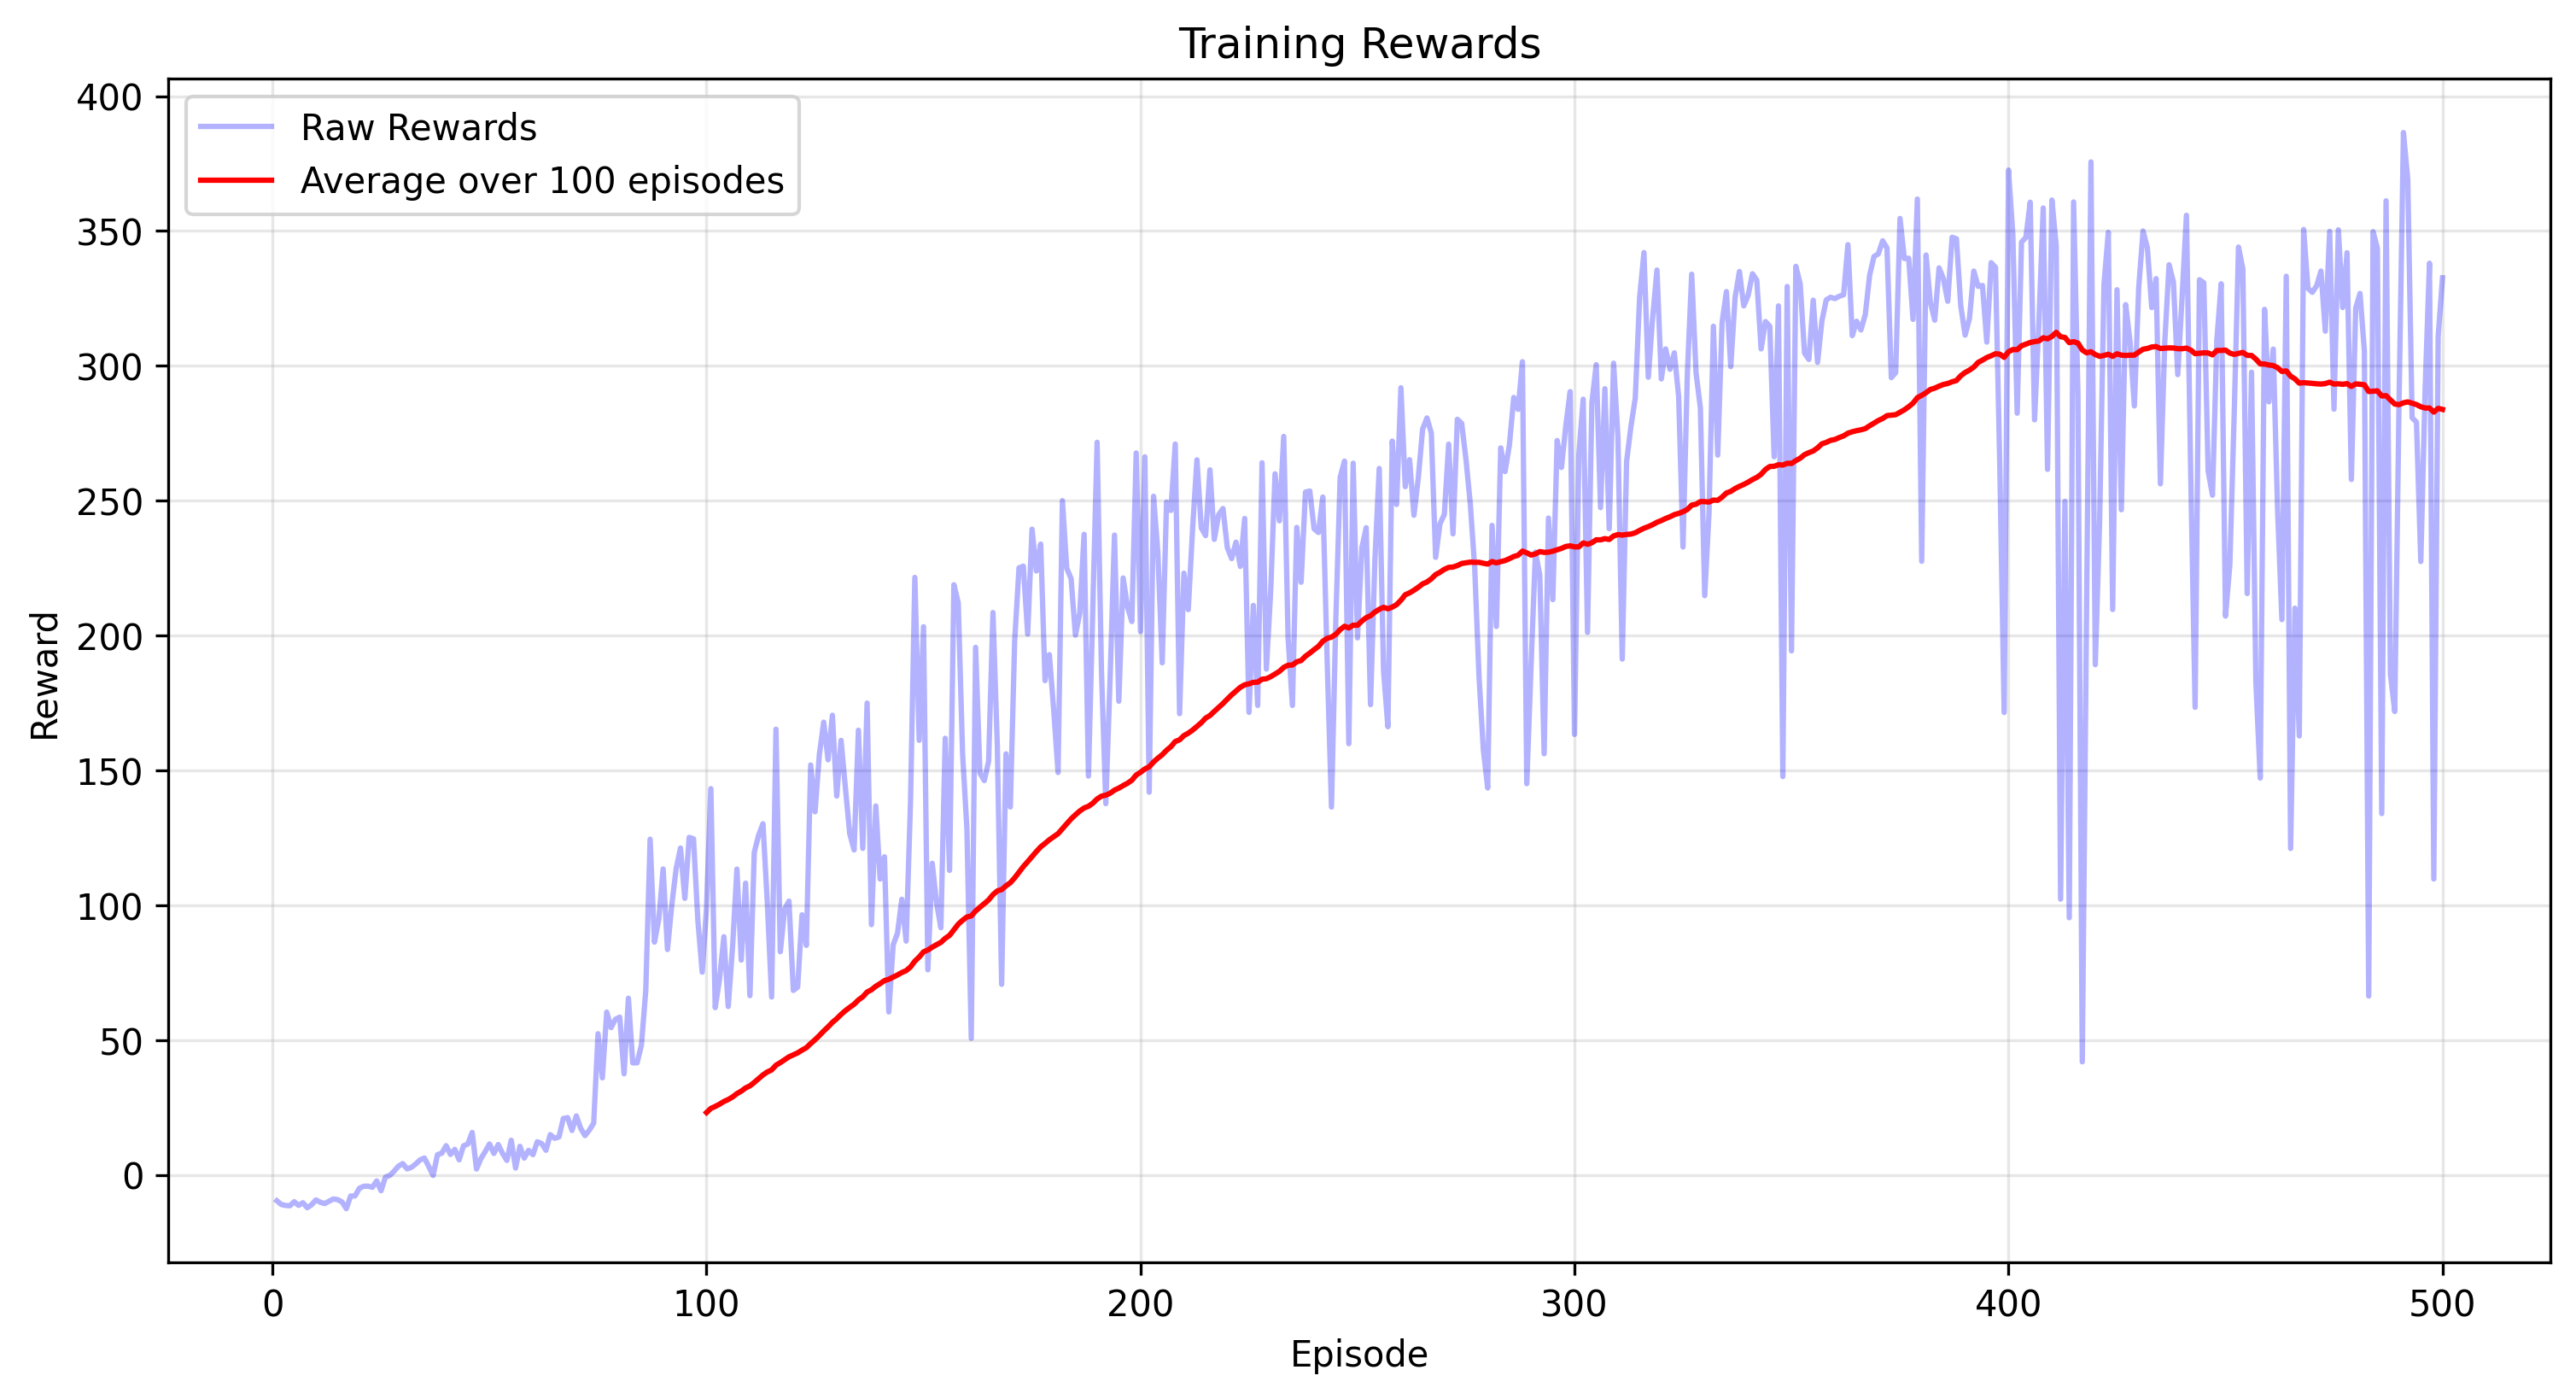
\includegraphics[width=0.7\textwidth]{mappo_training_rewards.png}
    \caption{MAPPO Training Rewards}
    \label{fig:mappo_rewards}
\end{figure}

The following are the results from the paper:

\begin{figure}[H]
    \centering
    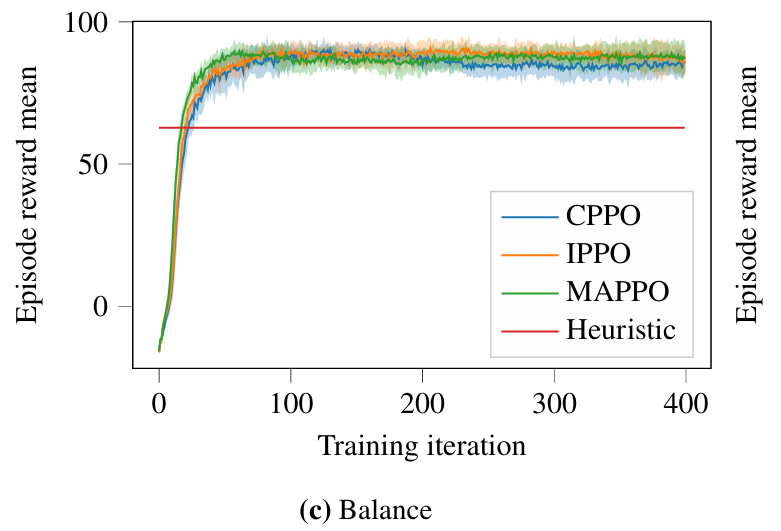
\includegraphics[width=0.7\textwidth]{training_rewards.png}
    \caption{Training Rewards from the Paper}
    \label{fig:paper_rewards}
\end{figure}

The specific training logs can be found in the root directory file \texttt{mappo\_training\_log.txt}. The trained models are also saved as \texttt{mappo\_best\_model.pth} and \texttt{mappo\_final\_model.pth}, which are located in the project root directory.

The results from the paper (\ref{fig:paper_rewards}) show faster convergence, stabilizing after approximately 50 iterations, with minimal fluctuations around a stable level of 90. In contrast, the reproduction results (\ref{fig:mappo_rewards}) exhibit slower convergence, requiring around 300 episodes to stabilize, with greater fluctuations after convergence. The raw rewards fluctuate between 100 and 350, while the average reward (red line) eventually stabilizes around 300.

\subsection{IPPO (Independent Learning PPO) - \texttt{train\_balance\_ippo.py}} 

\subsubsection{Actor Network Implementation}

\begin{verbatim}
class Actor(nn.Module):
    def __init__(self, obs_dim, action_dim, hidden_dim=256):
        super(Actor, self).__init__()
        # Feature extraction network
        self.net = nn.Sequential(
            nn.Linear(obs_dim, hidden_dim),
            nn.LayerNorm(hidden_dim),
            nn.Tanh(),
            nn.Linear(hidden_dim, hidden_dim),
            nn.LayerNorm(hidden_dim),
            nn.Tanh(),
            nn.Linear(hidden_dim, hidden_dim // 2),
            nn.LayerNorm(hidden_dim // 2),
            nn.Tanh(),
        )
        # Action distribution parameters layer
        self.mean_layer = nn.Linear(hidden_dim // 2, action_dim)
        self.log_std = nn.Parameter(torch.zeros(1, action_dim) - 1.0)
\end{verbatim}

\subsubsection{Critic Network Implementation}

\begin{verbatim}
class Critic(nn.Module):
    def __init__(self, obs_dim, hidden_dim=256):
        super(Critic, self).__init__()
        # Value estimation network
        self.net = nn.Sequential(
            nn.Linear(obs_dim, hidden_dim),
            nn.LayerNorm(hidden_dim),
            nn.Tanh(),
            nn.Linear(hidden_dim, hidden_dim),
            nn.LayerNorm(hidden_dim),
            nn.Tanh(),
            nn.Linear(hidden_dim, hidden_dim // 2),
            nn.LayerNorm(hidden_dim // 2),
            nn.Tanh(),
            nn.Linear(hidden_dim // 2, 1)
        )
\end{verbatim}

\subsubsection{Independent PPO Agent Implementation}

\begin{verbatim}
class IPPOAgent:
    def __init__(self, obs_dim, action_dim, agent_id, device="cpu"):
        self.device = device
        self.agent_id = agent_id
        
        # Create independent Actor and Critic networks
        self.actor = Actor(obs_dim, action_dim).to(device)
        self.critic = Critic(obs_dim).to(device)
        
        # Create optimizers
        self.actor_optimizer = optim.Adam(self.actor.parameters(), lr=3e-4)
        self.critic_optimizer = optim.Adam(self.critic.parameters(), lr=1e-3)
        
        # PPO hyperparameters
        self.clip_param = 0.2
        self.ppo_epochs = 10
        self.num_mini_batches = 4
        self.value_loss_coef = 0.5
        self.entropy_coef = 0.01
        self.max_grad_norm = 0.5
        self.gamma = 0.99
        self.gae_lambda = 0.95
\end{verbatim}

\subsubsection{Action Selection Implementation}

\begin{verbatim}
def select_action(self, obs):
    with torch.no_grad():
        # Get action distribution parameters
        mean, std = self.actor(obs)
        # Create normal distribution
        dist = Normal(mean, std)
        # Sample action
        action = dist.sample()
        action = torch.clamp(action, -1.0, 1.0)
        # Compute log probability and value
        log_prob = dist.log_prob(action).sum(-1, keepdim=True)
        value = self.critic(obs)
    return action, log_prob, value
\end{verbatim}

\subsubsection{GAE Calculation Implementation}

\begin{verbatim}
def compute_gae(self):
    T = len(self.rewards)
    num_envs = self.rewards[0].shape[0]
    advantages = torch.zeros(T, num_envs, 1, device=self.device)
    returns = torch.zeros(T, num_envs, 1, device=self.device)
    last_gae_lam = torch.zeros(num_envs, 1, device=self.device)
    
    # Reverse calculate GAE
    for t in reversed(range(T)):
        if t == T - 1:
            next_value = torch.zeros_like(self.values[0])
        else:
            next_value = self.values[t + 1]
        
        # Compute TD error
        delta = self.rewards[t] + self.gamma * next_value * (1 - \\
        self.dones[t]) - self.values[t]
        # Compute GAE
        advantages[t] = last_gae_lam = delta + self.gamma * \\
        self.gae_lambda * (1 - self.dones[t]) * last_gae_lam
        # Compute returns
        returns[t] = advantages[t] + self.values[t]
\end{verbatim}

\subsubsection{Policy Update Implementation}

\begin{verbatim}
def update(self):
    # Compute GAE
    advantages, returns = self.compute_gae()
    
    # Prepare data
    observations = torch.cat(self.observations)
    actions = torch.cat(self.actions)
    old_log_probs = torch.cat(self.log_probs)
    
    # Multiple policy iterations
    for i in range(self.ppo_epochs):
        # Compute new action distribution
        mean, std = self.actor(mb_obs)
        dist = Normal(mean, std)
        new_log_probs = dist.log_prob(mb_actions).sum(-1, keepdim=True)
        entropy = dist.entropy().mean()
        
        # Compute PPO objective
        ratio = torch.exp(new_log_probs - mb_old_log_probs)
        surr1 = ratio * mb_advantages
        surr2 = torch.clamp(ratio, 1.0 - self.clip_param, 1.0 + self.clip_param) * mb_advantages
        actor_loss = -torch.min(surr1, surr2).mean()
        
        # Compute value loss
        value_pred = self.critic(mb_obs)
        value_loss = 0.5 * ((mb_returns - value_pred) ** 2).mean()
        
        # Update networks
        self.actor_optimizer.zero_grad()
        actor_loss.backward()
        self.actor_optimizer.step()
        
        self.critic_optimizer.zero_grad()
        value_loss.backward()
        self.critic_optimizer.step()
\end{verbatim}

\subsubsection{Training Loop Implementation}

\begin{verbatim}
def train_episode(self):
    obs = self.env.reset()
    episode_reward = 0
    done = False
    
    while not done:
        # Each agent selects an action independently
        actions = []
        for i, agent in enumerate(self.agents):
            action, log_prob, value = agent.select_action(obs[i])
            actions.append(action)
            
            # Store transition data
            agent.store_transition(obs[i], action, rewards[i], value, \\
            log_prob, done)
        
        # Execute actions
        next_obs, rewards, dones, _ = self.env.step(actions)
        done = any(d.any() for d in dones)
        
        # Update observations
        obs = next_obs
        episode_reward += sum(r.mean().item() for r in rewards)
    
    # Independent updates for each agent
    for agent in self.agents:
        actor_loss, value_loss, entropy = agent.update()
\end{verbatim}

The following is the implementation process for the IPPO algorithm. The main features are as follows:

1. Independence:
   Each agent has its own Actor and Critic networks.
   Agents make independent decisions and learn independently.
   No parameters or information are shared between agents.

2. Parallel Training:
   Supports parallel sampling.
   Each agent learns simultaneously.
   Mini-batch training is used.

3. PPO Characteristics:
   Policy clipping is used to limit updates.
   GAE is applied to compute advantages.
   Entropy regularization is used to promote exploration.

4. Stability Optimizations:
   LayerNorm is used.
   Orthogonal initialization is applied.
   Gradient clipping is used.
   Advantage normalization is applied.

The reward curve is shown below:

\begin{figure}[H]
    \centering
    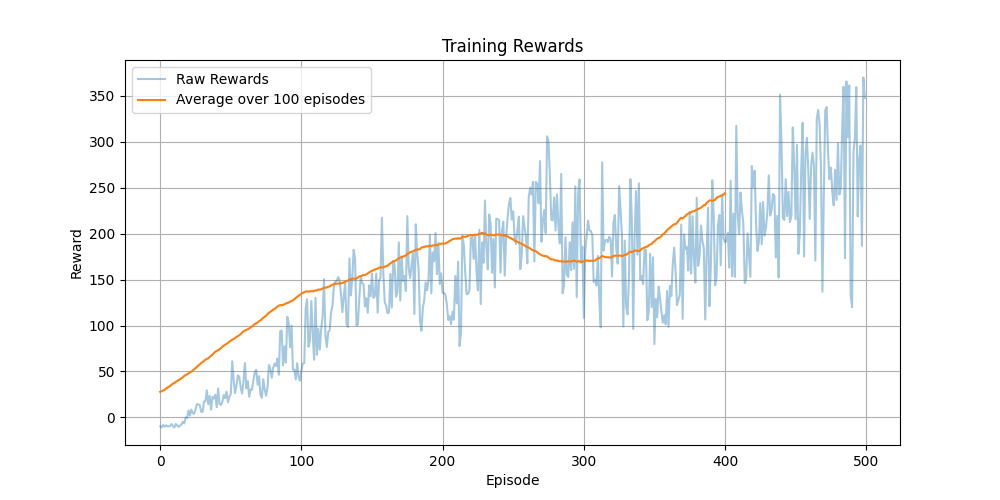
\includegraphics[width=0.8\textwidth]{ippo_training_rewards.png}
    \caption{IPPO Training Reward Curve}
    \label{fig:ippo_rewards}
\end{figure}

The following are the results from the paper:

\begin{figure}[H]
    \centering
    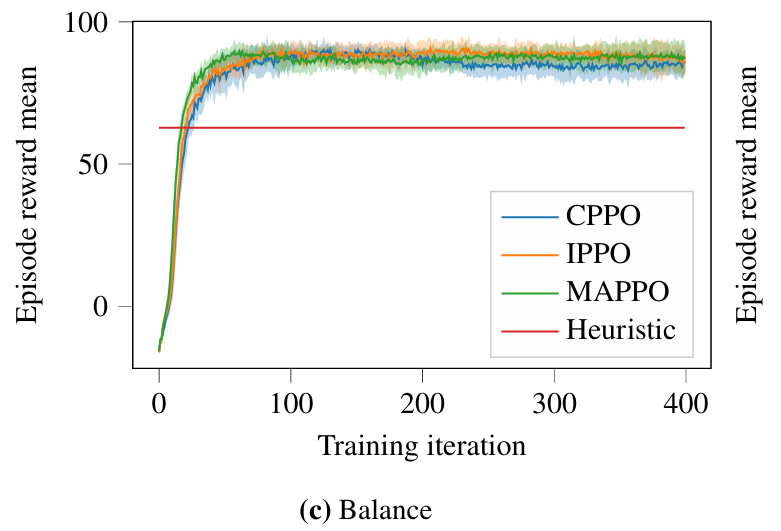
\includegraphics[width=0.8\textwidth]{training_rewards.png}
    \caption{Training Reward Curve from the Paper}
    \label{fig:paper_rewards}
\end{figure}

The specific training log can be found in the root directory file \texttt{ippo\_training\_log.txt}. The trained models are saved as \texttt{ippo\_best\_model.pth} and \texttt{ippo\_final\_model.pth}, which are also located in the project root directory.

Comparison and Analysis of the Two Reward Curves:
Results from the Paper (\ref{fig:paper_rewards}):Faster convergence, stabilizing after approximately 50 iterations.After convergence, minimal fluctuations, maintaining a stable level around 90.

Reproduction Results (\ref{fig:ippo_rewards}):Slower convergence, requiring around 200 episodes to start stabilizing.Raw Rewards fluctuate significantly, ranging from 100 to 350.The average reward (orange line) eventually stabilizes around 200, with a period of performance degradation (between episodes 250 and 300).



\section{Improvements to the IPPO Algorithm in \texttt{train\_balance\_ippo\_norm.py} and the Necessity and Superiority of the Improved Algorithm for the Task}

The main improvements of \texttt{train\_balance\_ippo\_norm.py} compared to \texttt{train\_balance\_ippo.py} are as follows:

\subsection{Addition of Observation Normalizer}
\begin{verbatim}
class ObservationNormalizer:
    def __init__(self, shape, device):
        self.running_mean = torch.zeros(shape).to(device)
        self.running_var = torch.ones(shape).to(device)
        self.count = 1e-4
\end{verbatim}

This is the primary improvement. It can: Calculate and update the mean and variance of observations in real time, Perform online normalization of input data, Use running averages to update statistics, ensuring stability.

\subsection{Integration of Normalization in the Agent Class}
\begin{verbatim}
def __init__(self, obs_dim, action_dim, agent_id, device="cpu"):
    # ...
    self.obs_normalizer = ObservationNormalizer(obs_dim, device)
\end{verbatim}

The normalizer instance is created during the agent initialization.

The normalized observations are used during action selection and policy updates.

\subsection{Improved Action Selection Process}
\begin{verbatim}
def select_action(self, obs):
    with torch.no_grad():
        normalized_obs = self.obs_normalizer.normalize(obs)
        mean, std = self.actor(normalized_obs)
        # ...
\end{verbatim}

Observations are normalized before action selection.

Ensures that the network receives more stable data distributions as inputs.

\subsection{Necessity and Superiority of the Improvements}

The necessity and superiority of the improvements can be reflected in the following points:

\subsubsection{Training Stability}

Normalization ensures that observations from different dimensions are scaled to similar ranges.Prevents gradient issues caused by some dimensions having disproportionately large or small values.Reduces numerical instability during the training process.

\subsubsection{Learning Efficiency}
A normalized data distribution is more conducive to neural network learning.Accelerates the convergence of the network.Reduces training difficulties due to inconsistent value ranges across input features.

\subsubsection{Generalization Ability}Normalization makes the model more responsive to inputs with different scales.Enhances the model's ability to adapt to different environmental states.

\subsubsection{Analyse}
The Analyse is as follows:

Before Improvement:

\begin{figure}[H]
    \centering
    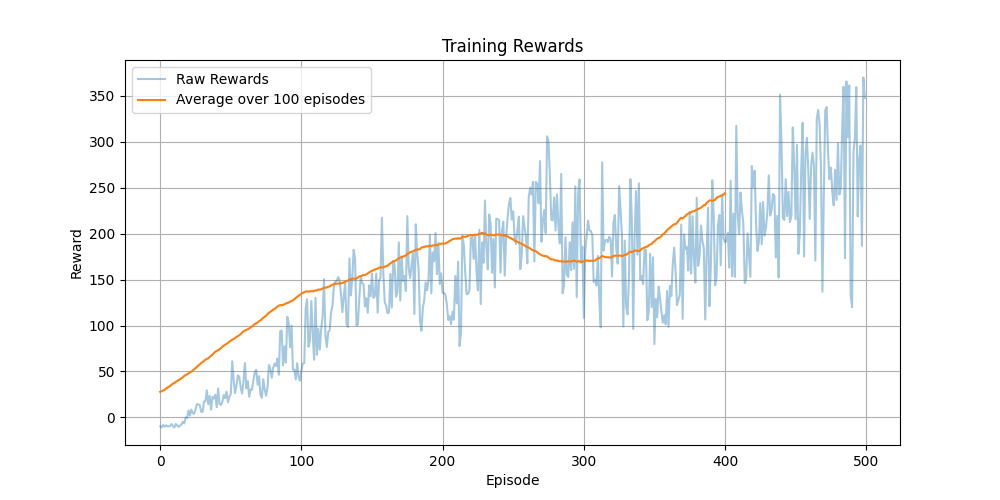
\includegraphics[width=0.8\textwidth]{ippo_training_rewards.png}
    \caption{IPPO Training Reward Curve (Before Improvement)}
    \label{fig:ippo_rewards_before}
\end{figure}

After Improvement:

\begin{figure}[H]
    \centering
    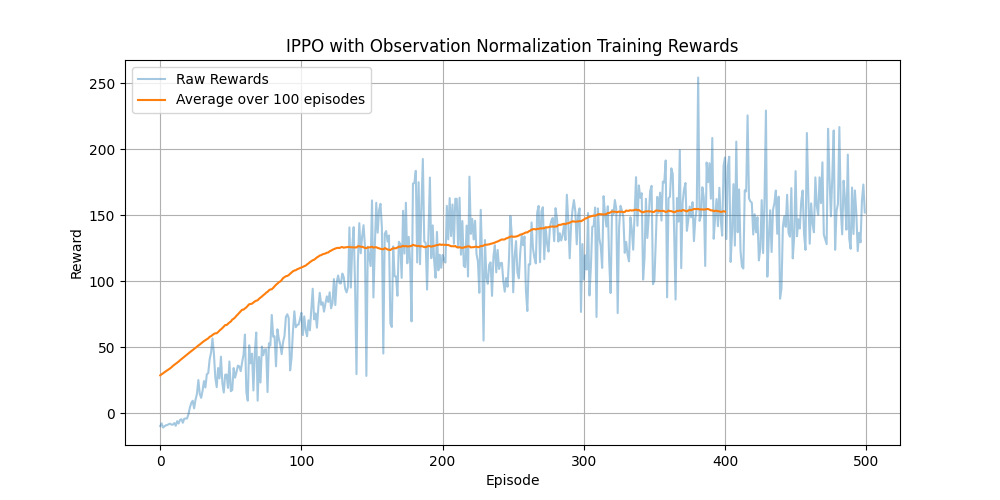
\includegraphics[width=0.8\textwidth]{ippo_norm_training_rewards.png}
    \caption{IPPO Normalized Training Reward Curve (After Improvement)}
    \label{fig:ippo_rewards_after}
\end{figure}

The specific training log can be found in the root directory file \texttt{ippo\_norm\_training\_log.txt}. The trained models are saved as \texttt{ippo\_norm\_best\_model.pth} and \texttt{ippo\_norm\_final\_model.pth}, which are also located in the project root directory.

As observed, after the improvement, the convergence speed has increased and the training has become more stable.

\section{Discussion on the Impact of the Number of Agents on Experimental Results}

\subsection{System Complexity}
The number of agents directly impacts the dimensionality of the state and action spaces.More agents require more complex interactions.Each agent must process the state information of other agents, causing the computational complexity to rise significantly as the number of agents increases.

\subsection{Training Efficiency}
Increasing the number of agents leads to longer training times.More computational resources are required to handle the parallel environment.Each agent’s policy update needs to take into account the behaviors of other agents, which reduces the convergence speed.

\subsection{Change in the Observation Space}
\begin{verbatim}
def observation(self, agent):
    # The observation space changes with the number of agents.
    # Each agent needs to process more relative state information.
    observation = self.scenario.observation(agent)
\end{verbatim}

\subsection{Reward Allocation}
In multi-agent systems, reward allocation becomes more complex.A balance must be found between individual rewards and team rewards.

\section{GitHub Project Repository}

\url{https://github.com/Jaywang2924718196/VmasRepetition/tree/master}


\end{document}
